\begin{center}
  \Large
  \textbf{AUTHOR'S BIOGRAPHY}
\end{center}

\addcontentsline{toc}{chapter}{AUTHOR'S BIOGRAPHY}

\vspace{2ex}

\begin{wrapfigure}{L}{0.3\textwidth}
  \centering
  \vspace{-3ex}
  % Ubah file gambar berikut dengan file foto dari mahasiswa
  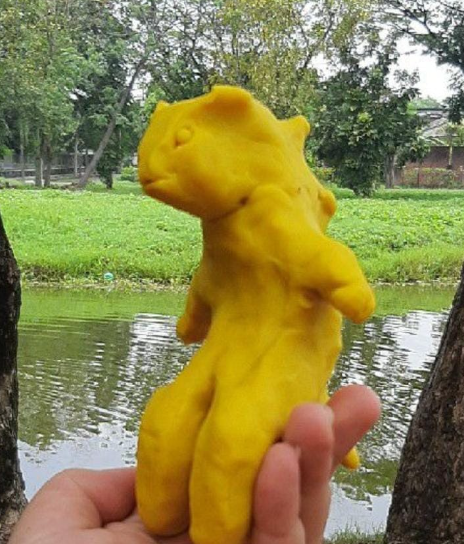
\includegraphics[width=0.3\textwidth]{figures/yellow.png}
  \vspace{-4ex}
\end{wrapfigure}

% Ubah kalimat berikut dengan biografi dari mahasiswa
\name{}, born on the day he was born, was a creature with many interests.
\lipsum[1-2]
%He began his journey on exploring computer science and engineering (CSE) when he was in his third year of middle school.
%He found a random C programming language book in a bookstore, bought it, read it, and created his first hello world right after.
%
%His training arc for CSE started in high school. 
%Due to an unknown reason, his homeroom teacher forced him to enroll in the high school's mathematics olympiad team.
%As he was a pushover back then, he just followed what his teacher said.
%Fortunately, the math teacher didn't really want to teach olympiad level math, and recommended him to try informatics olympiad instead.
%That's how he met his master who taught him the competitive programming 101.


%\lipsum[1]

%\lipsum[2]
